% Tõlge: Katrin Gabrel, Ahto Truu

\documentclass[a4paper,11pt]{article}
\usepackage[et]{../../eio}

\usepackage{tikz}
\tikzset{every picture/.style = {thick, scale=0.5}}
\tikzset{uno/.style = {fill, shape=circle, inner sep=2}}
\tikzset{post/.style = {fill, shape=circle, inner sep=1}}
\tikzset{label/.style = {black, midway}}

\begin{document}
\begin{ol}{\eio}{\vv 19.04.2020}{\lah}{}
\begin{yl}{1}{Aed}{aed}{1 sek / 3 sek}{100 punkti}

Tasandil on $N$ tipuga hulknurk ja punkt $U$, mis võib olla nii hulknurga sees kui sellest väljas. Leida, milliseid hulknurga külgi punktis $U$ olev vaatleja näeb.

Ülesande lahendamiseks võime vaadelda hulknurga iga külge (alloleval joonisel sinine) eraldi ja uurida, kas mingi osa sellest on vaatlejale nähtav. Nähtavat osa võime arvestada sektorina (punane), mida hulknurga ülejäänud külgi (mustad) järjest läbi vaadates jooksvalt kitsendame.

\begin{center}
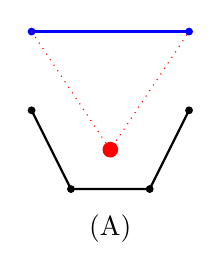
\begin{tikzpicture}
  \draw[blue] (1, 4) node[post]{}
    -- (5, 4) node[post]{};
  \draw[red, thin, dotted] (1, 4)
    -- (3, 1) node[uno]{}
    -- (5, 4);
  \draw[black] (1, 2) node[post]{}
    -- (2, 0) node[post]{}
    -- (4, 0) node[post]{}
    -- (5, 2) node[post]{};
  \draw (3, -1) node{(A)};
\end{tikzpicture}
\hskip 1cm
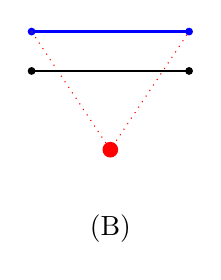
\begin{tikzpicture}
  \draw[blue] (1, 4) node[post]{}
    -- (5, 4) node[post]{};
  \draw[red, thin, dotted] (1, 4)
    -- (3, 1) node[uno]{}
    -- (5, 4);
  \draw[black] (1, 3) node[post]{}
    -- (5, 3) node[post]{};
  \draw (3, -1) node{(B)};
\end{tikzpicture}
\hskip 1cm
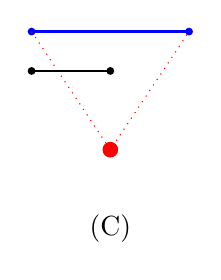
\begin{tikzpicture}
  \draw[blue] (1, 4) node[post]{}
    -- (5, 4) node[post]{};
  \draw[red, thin, dotted] (1, 4)
    -- (3, 1) node[uno]{}
    -- (5, 4);
  \draw[black] (1, 3) node[post]{}
    -- (3, 3) node[post]{};
  \draw (3, -1) node{(C)};
\end{tikzpicture}
\hskip 1cm
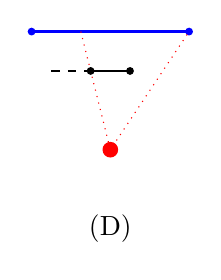
\begin{tikzpicture}
  \draw[blue] (1, 4) node[post]{}
    -- (5, 4) node[post]{};
  \draw[red, thin, dotted] (2.25, 4)
    -- (3, 1) node[uno]{}
    -- (5, 4);
  \draw[black, dashed] (1.5, 3) -- (2.5, 3);
  \draw[black] (2.5, 3) node[post]{}
    -- (3.5, 3) node[post]{};
  \draw (3, -1) node{(D)};
\end{tikzpicture}
\end{center}

Kui hulknurga ülejäänud külgi läbida vaadeldava külje ühest otsast alates ja mööda hulknurga piirjoont edasi liikudes, siis võib iga järgmine külg olla kas täiesti väljaspool vaatesektorit (A), läbida sektori (B) või olla sektoris ainult ühte otsa pidi (C).

Oluline on, et varjav külg ei saa olla tervenisti sektori sisemuses, sest siis pidi ka sellele eelnev külg vähemalt osaliselt sektori sees olema ja oleks seda kitsendanud (D). See tähendab, et nähtav sektor püsib kogu protsessi vältel sidusana ja me saame selle üle arvet pidada kahe kiirega.

Kiire ja lõigu vastastikuse asendi tuvastamiseks võime kasutada vektorkorrutise omadusi. Tasandi vektorite $\vec{u} = (x_u, y_u)$ ja $\vec{v} = (x_v, y_v)$ vektorkorrutis $\vec{u} \times \vec{v} = x_u \cdot y_v - x_v \cdot y_u$ on positiivne, kui pööre vektori $\vec{u}$ suunalt vektori $\vec{v}$ suunale on vastupäeva (alloleval joonisel vasakul), ja negatiivne, kui pööre on päripäeva.\footnote{Tegelikult on vektorkorrutis ruumivektorite vahel defineeritud tehe, mille tulemus on samuti ruumivektor. Aga kuna tasandivektorite vektorkorrutise $x$- ja $y$-koordinaadid on alati nullid, siis kasutatakse tasandi geomeetria ülesannetes vektorkorrutise asemel selle $z$-koordinaadi väärtust.} See tähendab, et punkte $p_1$ ja $p_2$ läbiv sirge lõikab punkte $q_1$ ja $q_2$ ühendavat lõiku parajasti siis, kui $\vec{p_1 p_2} \times \vec{p_1 q_1}$ ja $\vec{p_1 p_2} \times \vec{p_1 q_2}$ on erimärgilised (joonisel paremal).

\begin{center}
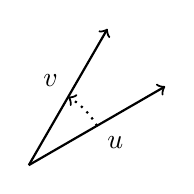
\begin{tikzpicture}
  \draw[->] (0, 0) -- (30 : 4) node[label, below right]{$u$};
  \draw[->] (0, 0) -- (60 : 4) node[label, above left]{$v$};
  \draw[->, dotted] (30 : 2) arc[radius = 2, start angle = 30, end angle = 60];
\end{tikzpicture}
\hskip 3cm
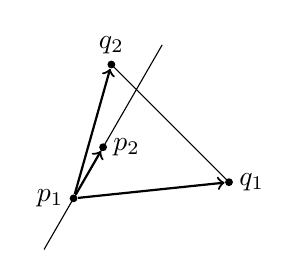
\begin{tikzpicture}
  \draw[thin] (0, 0) -- (60 : 6)
    node(p1)[near start, post]{}
    node(p2)[midway, post]{};
  \draw[thin] (20 : 5) node(q1)[post]{}
    -- (70: 5) node(q2)[post]{};
  \draw[->] (p1) node[left]{$p_1$}
    -- (p2) node[right]{$p_2$};
  \draw[->] (p1)
    -- (q1) node[right]{$q_1$};
  \draw[->] (p1)
    -- (q2) node[above]{$q_2$};
\end{tikzpicture}
\end{center}

Lisaks vaatesihiga lõikumise faktile on vaja teada ka seda, kas potentsiaalselt varjav lõik on vaatleja ja vaadeldava lõigu vahel. Lõikepunkti kauguse punktist $p_1$ saame avaldada järgmistest tähelepanekutest.

Kõik punkte $p_1$ ja $p_2$ läbival sirgel asuvad punktid $p$ avalduvad kujul $p = p_1 + t \cdot \vec{p_1 p_2}$. Samamoodi avalduvad sirge $q_1 q_2$ punktid kujul $q_1 + u \cdot \vec{q_1 q_2}$. Lõikepunkt peab rahuldama mõlemat võrrandit. Seega otsime $t$ ja $u$ väärtusi, mille korral
  \[
    p_1 + t \cdot \vec{p_1 p_2} = q_1 + u \cdot \vec{q_1 q_2}
  \]
ehk koordinaatide kaupa välja kirjutades
  \[
    \left\{
    \begin{aligned}
      x_{p_1} + t \cdot (x_{p_2} - x_{p_1}) &= x_{q_1} + u \cdot (x_{q_2} - x_{q_1}) \\
      y_{p_1} + t \cdot (y_{p_2} - y_{p_1}) &= y_{q_1} + u \cdot (y_{q_2} - y_{q_1})
    \end{aligned}
    \right. \; ,
  \]
millest esimest võrrandit $(y_{q_2} - y_{q_1})$-ga ja teist võrrandit $(x_{q_2} - x_{q_1})$-ga korrutades, neid üksteisest lahutades ja siis sarnaseid liikmeid koondades saame avaldada
  \begin{equation} \label{eqn:t}
    t = \frac{(x_{q_1} - x_{p_1}) \cdot (y_{q_2} - y_{q_1}) - (y_{q_1} - y_{p_1}) \cdot (x_{q_2} - x_{q_1})}
            {(x_{p_2} - x_{p_1}) \cdot (y_{q_2} - y_{q_1}) - (y_{p_2} - y_{p_1}) \cdot (x_{q_2} - x_{q_1})}
      = \frac{\vec{p_1 q_1} \times \vec{q_1 q_2}}{\vec{p_1 p_2} \times \vec{q_1 q_2}} \; .
  \end{equation}
Nüüd saaksime avaldada lõikepunkti kauguse punktist $p_1$ kujul $d = t \cdot |p_1 p_2|$, aga seda pole tegelikult vaja. Piisab tähelepanekust, et $t < 0$ vastab punktidele, mis on sirgel punktist $p_2$ vaadates teisel pool punkti $p_1$, $0 < t < 1$ vastab punktidele, mis on $p_1$ ja $p_2$ vahel, ning $t > 1$ vastab punktidele, mis on punktist $p_1$ vaadates teisel pool punkti $p_2$. Sisuliselt annab $t$ väärtus meile lõikepunkti koordinaadi teljel, kus $\vec{p_1 p_2}$ on ühikvektor, ja me võime erinevate lõikepunktide omavahelisi asendeid uurida neile vastavate $t$ väärtuste võrdlemise teel.

Absoluutarvudes kauguste asemel $t$ väärtuste kasutamisel on üks põhimõtteline eelis: kui punktide koordinaadid on täisarvud, siis on valemist~(\ref{eqn:t}) saadud $t$ väärtused alati ratsionaalarvud, mida võime programmis hoida harilike murdudena ja mille võrdlemine on sel juhul täpne, ümardamisvigadeta. Nii ongi tehtud Pythoni lahenduses failis \verb'sol.py'.

Praktiliselt on selles ülesandes võimalik saada kõigis testides õiged vastused ka topelttäpsusega reaalarve kasutades, nagu on tehtud C++ lahenduses failis \verb'sol.cpp', kus valenegatiivsete tulemuste vältimiseks võrreldakse arve teatud täpsuspiirini: üksteisest vähem kui $10^{-6}$ võrra erinevad arvud loetakse võrdseks.

Pythoni harilike murdudega lahendust C++ ümber kirjutades peaks olema ettevaatlik. Nimelt võivad murdudega arvutades nende nimetajad ja lugejad C++ piiratud suurusega (32 või 64 bitti) täisarvutüüpides ületäitumisi põhjustada. Pythonis seda ohtu ei ole, sest Python läheb väärtuste kasvades automaatselt üle ülipikkade täisarvude kasutamisele.

Teiselt poolt väärib mainimist, et nii Pythoni kui C++ täisarvudes ja ka Pythoni ujukomaarvudes põhjustab nulliga jagamise katse alati veaolukorra, aga C++ ujukomaarvudes annab positiivse või negatiivse arvu nulliga jagamine tulemuseks vastavalt $+\infty$ või $-\infty$.\footnote{Selline käitumine ei ole C++ standardi järgi kohustuslik. See on aga lubatud laiendus ja olümpiaadi serveris lahenduste testimiseks kasutatav kompilaator nii käitub.} Nende ebanormaalsete väärtustega edasi arvutades peab küll ettevaatlik olema, aga siiski võimaldab see sageli koodi märgatavalt lihtsustada.

\end{yl}
\end{ol}
\end{document}
